\documentclass[14pt]{beamer}

\mode<presentation> {
\usetheme{Madrid}

% To remove the navigation symbols from the bottom of all slides uncomment next line
\setbeamertemplate{navigation symbols}{} 
\date{}
\title{}
\author{}

%to get rid of footer entirely uncomment next line
\setbeamertemplate{footline}{}
}


\usepackage{geometry}
\usepackage{multirow}
\usepackage{adjustbox}
\usepackage{multicol}
\setlength{\columnsep}{0.1cm}


\usepackage{tikz}
\usetikzlibrary{shapes,backgrounds}

\usepackage{bbding}
\usepackage{rotating}
\usepackage{xcolor}


%\usepackage{tkz-berge} %cool grid
\usepackage{pgfplots} %pics

\usepackage{graphicx} % Allows including images
\usepackage{booktabs} % Allows the use of \toprule, \midrule and \bottomrule in tables
\usepackage{mathtools}

\newcommand {\DS} [1] {${\displaystyle #1}$}
\newcommand {\R}{\mathbb{R}}
\newcommand {\Z}{\mathbb{Z}}
\newcommand {\N}{\mathbb{N}}
\newcommand{\e}{\varepsilon}

\newcommand{\p}{\pause}

% simple environrment for enumerate, easier to read
\setbeamertemplate{enumerate items}[default]

%%%%%%%%%%%%%%%%%%%%%%

% to use colours easily
\definecolor{verde}{rgb}{0, .7, 0} 
\definecolor{rosa}{rgb}{1, 0, 1}  
\definecolor{naranja}{rgb}{1, .5, 0.1} 
\newcommand{\azul}[1]{{\color{blue} #1}}
\newcommand{\rojo}[1]{{\color{red} #1}}
\newcommand{\verde}[1]{{\color{verde} #1}}
\newcommand{\rosa}[1]{{\color{rosa} #1}}
\newcommand{\naranja}[1]{{\color{naranja} #1}}
\newcommand{\violeta}[1]{{\color{violet} #1}}
 
% box in red and blue in math and outside of math
\newcommand{\cajar}[1]{\boxed{\mbox{\rojo{ #1}}}}
\newcommand{\majar}[1]{\boxed{\rojo{ #1}}}
\newcommand{\cajab}[1]{\boxed{\mbox{\azul{ #1}}}}
\newcommand{\majab}[1]{\boxed{\azul{ #1}}}
 
\newcommand{\setsize}[1]{\fontsize{#1}{#1}\selectfont} %allows you to change the font size. The default size of this document is 14. To change the font size of the whole slide, place this at the beginning of the slide. To change the size of only a portion of the text to size 12, you can do the following { \setsize{12} Your text. }.

\setbeamerfont{frametitle}{size=\setsize{15}}
\setbeamerfont{block title}{size=\setsize{14}}

\newcommand{\smallerfont}{\setsize{13}} %place this at the beginning of a slide to set the font size of the entire slide to 13.

%===========================
% Preamble just for this file
%===========================


\newcommand{\erf}{\operatorname{erf}}
\newcommand{\vv}{\vspace{.1cm}}

%===================================================
\begin{document}
%===================================================

%----------------------------------------------------------------------------------------
%	Antiderivatives
%----------------------------------------------------------------------------------------
%-----------------------------
\begin{frame}[t]
\frametitle{Initial Value Problem}

Find a function $f$ such that
	\begin{itemize}
		\item  For every \DS{x \in \R},  \DS{f''(x) = \sin x + x^2},
		\item  \DS{f'(0) = 5},
		\item  \DS{f(0) = 7}.
	\end{itemize}

\end{frame}
%-----------------------------
\begin{frame}[t]
\smallerfont
\frametitle{The most misunderstood antiderivative}
\begin{enumerate}
	\item Find the \emph{domain} and the derivative of \; \DS{F_1(x) = \ln x}
		\vv
	\item Find the \emph{domain} and the derivative of \; \DS{F_2(x) = \ln (-x)}
		\vv
	\item Find the \emph{domain} and the derivative of \; \DS{F_3(x) = \ln |x|}
		\vv
		
		\emph{Suggestion:}  Break the domain into two pieces.
		\vv
\p
	\item \label{qu:ln} Based on your answers, what is \DS{\int \frac{1}{x} \,dx \,}?
		\vv
\p 
	\item Find the \emph{domain} and the derivative of \; \DS{F_4(x) = \ln |2x|}
		\vv
	
		Why doesn't this contradict your answer to \azul{4} ?
\end{enumerate}

\end{frame}
%-----------------------------
\begin{frame}[t]
\smallerfont
\frametitle{Compute these antiderivatives by guess 'n check}

\begin{enumerate}
\begin{multicols}{2}
	\item \DS{\int x^5 dx}
	\item  \DS{\int \left( 3x^8 -18x^5 + 1 \right) dx}
	\item \DS{\int \sqrt[3]{x} \; dx}
	\item \DS{\int \frac{1}{x^9} \;dx}
	\item \DS{\int \sqrt{x}\left( x^2+ 5 \right) dx}
	\item \DS{\int \frac{1}{e^{2x}} \; dx}
	\item \DS{\int \sin (3x) \; dx}
	\item \DS{\int \cos (3x+2) \;dx}
	\item \DS{\int \sec^2 x \;dx}
	\item \DS{\int \sec x \tan x \; dx}
	\item \DS{\int \frac{1}{x} \; dx}
	\item \DS{\int \frac{1}{x+3} \; dx}
\end{multicols}
\end{enumerate}

\end{frame}
%-----------------------------
\begin{frame}[t]
\frametitle{Integration by parts 1}

\begin{enumerate}
	\item  \DS{\frac{d}{dx} \left[ x \sin x \right] = }
	\vv \vv
	\item \DS{\frac{d}{dx} \left[ \cos x \right] = }
	\vv \vv
\end{enumerate}
\vv \vv
Use the previous answers to calculate
\vv \vv
\begin{enumerate}
\addtocounter{enumi}{2}
	\item \DS{\int x \cos x \, dx = }
\end{enumerate}

\end{frame}
%-----------------------------
\begin{frame}[t]
\frametitle{Integration by parts 2}

\begin{enumerate}
	\item  \DS{\frac{d}{dx} \left[ x e^x \right] = }
	\vspace{.5cm}
	\item \DS{???  }
	\vspace{.5cm}
	\item \DS{\int x e^x \, dx = }
\end{enumerate}

\end{frame}
%-----------------------------
\begin{frame}[t]
\frametitle{Integration by parts 3}

\begin{enumerate}
	\item \DS{???  }
	\vspace{.3cm}
	\item \DS{???  }
	\vspace{.3cm}
	\item \DS{\int x e^{-x} \, dx = }
\end{enumerate}

\end{frame}
%-----------------------------
\begin{frame}[t]
\frametitle{Integration by parts 4}

\begin{enumerate}
	\item  \DS{\frac{d}{dx} \left[ x^2 e^x \right] = }
	\vv \vv
	\item  \DS{\frac{d}{dx} \left[ x e^x \right] = }
	\vspace{.5cm}
	\item \DS{???  }
	\vspace{.5cm}
	\item \DS{\int x^2 e^x \, dx = }
\end{enumerate}

\end{frame}
%-----------------------------
\begin{frame}[t]
\frametitle{Trig-exp antiderivatives}

\begin{enumerate}
	\item \DS{\frac{d}{dx} \left[ e^x \sin x \right]=}
	\vv \vv
	\item \DS{\frac{d}{dx} \left[ e^x \cos x \right]=}
\end{enumerate}
\vspace{.5cm}
Use the previous answers to calculate:
\vspace{.3cm}
\begin{enumerate}
\addtocounter{enumi}{2}
	\item \DS{\int e^x \sin x \, dx = }
	\vv \vv
	\item \DS{\int e^x \cos x \, dx = }
\end{enumerate}

\end{frame}
%-----------------------------
\begin{frame}[t]
\frametitle{A challenge for guess-and-check ninjas}
	$$
		\int x \, e^x \cos x \, dx \; = \; \; ???
	$$

\end{frame}
%-----------------------------
%----------------------------------------------------------------------------------------
%	Functions defined as integrals
%----------------------------------------------------------------------------------------
%-----------------------------
\begin{frame}[t]
\setsize{11}
\frametitle{Functions defined by integrals}
 
 Which ones of these are valid ways to define functions?

		\vv
 
 \begin{multicols}{2}
\begin{enumerate}
	\item \DS{F(x) = \int_0^x \frac{t}{1+ t^8} \; dt}
		\vspace{.3cm}
	\item \DS{F(x) = \int_0^x \frac{x}{1+ x^8} \;  dx}
		\vspace{.3cm}
	\item \DS{F(x) = \int_0^x \frac{x}{1+ t^8} \;  dt}
		\vspace{.3cm}
	\item \DS{F(x) = \int_0^{x^2} \frac{t}{1+t^8} \;  dt}
		\vspace{.3cm}
	\item \DS{F(x) = \int_{\sin x}^{e^x} \frac{t}{1+t^8} \;  dt}
		\vspace{.3cm}
	\item \DS{F(x) = \int_0^3 \frac{t}{1+x^2+t^8} \;  dt}
		\vspace{.3cm}
	\item \DS{F(x) =  x \int_{\sin x}^{e^x} \frac{t}{1+x^2+t^8} \;  dt}
		\vspace{.3cm}
	\item \DS{F(x) =  t \int_{\sin x}^{e^x} \frac{t}{1+x^2+t^8} \;  dt}
		\vspace{.3cm}
\end{enumerate}
\end{multicols}

\end{frame}
%------------------------------
\begin{frame}[t]
\frametitle{Towards FTC}

\begin{columns}

\begin{column}{.7\textwidth}
\begin{center}
	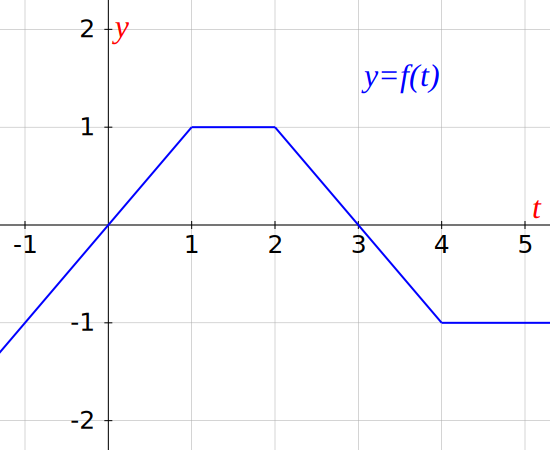
\includegraphics[scale=.4]{G21}
\end{center}
\end{column}

\begin{column}{.3\textwidth}
Compute:
	\begin{enumerate}
		\item  \DS{\int_0^1 \! f(t) dt}
		\item  \DS{\int_0^2 \! f(t) dt}
		\item  \DS{\int_0^3 \! f(t) dt}
		\item  \DS{\int_0^4 \! f(t) dt}
		\item  \DS{\int_0^5 \! f(t) dt}
	\end{enumerate}
\end{column}
\end{columns}

\end{frame}
%------------------------------
\begin{frame}[t]
\smallerfont
\frametitle{Towards FTC (continued)}

\begin{center}
	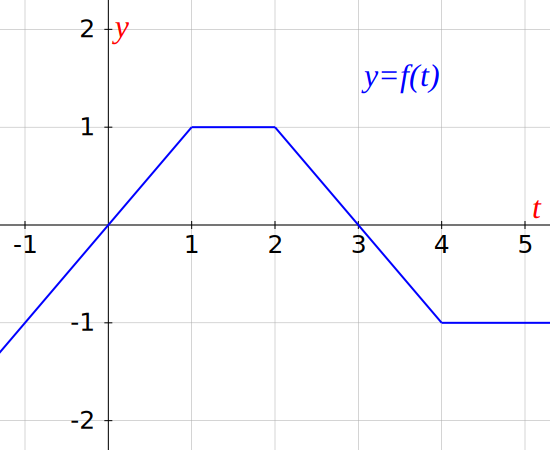
\includegraphics[width=8cm, height=5cm]{G21}
\end{center}

Call \DS{F(x) = \int_0^x f(t) dt}.  This is a new function. 
\begin{itemize}
	\item Sketch the graph of \DS{y=F(x)}.  
	\item  Using the graph you just sketched, sketch the graph of \DS{y=F'(x)}.
\end{itemize}
\end{frame}

%-----------------------------
%----------------------------------------------------------------------------------------
%	FTC - 1
%----------------------------------------------------------------------------------------
%------------------------------
\begin{frame}[t]
\frametitle{Filling the tank}

A tank is being filled with water.  At time $t$ water flows into the tank at a rate of
	$$
		A \, e^{-bt} \arctan (ct) 
	$$
litres per second, where $A$, $b$, and $c$ are constants.  The amount of water in the tank at time $t=0s$  is $V_0$.  Write an expression for the amount of water $V$ in the tank at time $t$.


\end{frame}
%-----------------------------
\begin{frame}[t]
\smallerfont
\frametitle{True or False?}

\begin{enumerate}
\item If $f$ is continuous on the interval $[a,b]$, then 
	$$\frac{d}{dx}\left( \int_a^b f(t)dt\right)=f(x).$$

\vspace{4mm}

\item If $f$ is differentiable, then 
	$$
		\frac{d}{dx} \left(\int_a^x f(t)\,dt \right) \; = \;   \int_a^x f'(t) \,dt .
	$$
 
\end{enumerate}

\end{frame}
%-----------------------------
\begin{frame}[t]
\smallerfont
\frametitle{More True or False}

Let $f$ and $g$ be differentiable functions with domain \DS{\R}.  \\
Assume that \DS{f'(x) = g(x)} for all $x$.  \\
Which of the following statements must be true?

	\begin{enumerate}
		\item  \DS{f(x) = \int_0^x g(t) dt}. 
		
						
		\item  If \DS{f(0)=0}, then \DS{f(x) = \int_0^x g(t) dt}.  
		
		
		\item  If \DS{g(0)=0}, then \DS{f(x) = \int_0^x g(t) dt}. 
		
		
		\item There exists $C \in \mathbb{R}$ such that \DS{f(x) = C + \int_0^x g(t) dt}.  
		
		
		\item  There exists $C\in \mathbb{R}$ such that \DS{f(x) = C + \int_1^x g(t) dt}.  
				
	\end{enumerate}
\end{frame}
%-----------------------------
\begin{frame}[t]
\setsize{11}
\frametitle{True, False, or Shrug?}

We want to find a function $H$ with domain $\R$ such that \DS{H(1) = -2} and such that
		  \DS{H'(x) = e^{\sin x}} for all $x$.
Decide whether each of the following statements is true, false, or we do not have enough information to decide. 

\begin{enumerate}
	\item  The function \DS{\quad H(x) = \int_0^x e^{\sin t} dt \quad} is a solution.
	\item  The function \DS{\quad H(x) = \int_2^x e^{\sin t} dt \quad} is a solution.
	\item $\forall C \in \R$, the function  \DS{\quad H(x) = \int_0^x e^{\sin t} dt + C \quad} is a solution. 
	\item $\exists C \in \R$ s.t.\ the function \DS{\quad H(x) = \int_0^x e^{\sin t} dt + C \quad } is a solution.
	\item The function \DS{\quad H(x) = \int_1^x e^{\sin t} dt -2 \quad} is a solution.
	\item There is more than one solution.
\end{enumerate}

\end{frame}
%------------------------------
\begin{frame}[t]
\smallerfont
\frametitle{Examples of FTC-1}

Compute the derivative of the following functions

	\begin{enumerate}
		\item  \DS{F_1(x) = \int_0^1 e^{-t^2} dt}. \\
	\vfill 
				
		\item   \DS{F_2(x) = \int_0^x e^{-\sin t} dt}. \\
	\vfill 
		
		\item  \DS{F_3(x) = \int_1^{x^2} \frac{\sin t}{t^2} dt}. \\
	\vfill 
		
		\item  \DS{F_4(x) = \! \int_x^7 \sin^3 \! \! \left( \sqrt{t} \right) \! dt}. \\
	\vfill 
		
		\item  \DS{F_5(x) = \int_{2x}^{x^2} \frac{1}{1+t^3} dt}. \\
	\end{enumerate}

\end{frame}
%------------------------------
\begin{frame}[t]
\frametitle{A generalized version of FTC-1}

Let $f$, $u$, $v$ be differentiable functions with domain $\R$.
Let us call
	$$
		F(x) = \int_{u(x)}^{v(x)} f(t) dt
	$$
Find a formula for 
	$$
		F'(x)
	$$
in terms of $f$, $u$, $v$, $f'$, $u'$, $v'$.

\end{frame}

%------------------------------
\begin{frame}[t]
\frametitle{An integral equation}

Assume $f$ is a continuous function that satisfies, for every $x \in \R$:
	$$
		\int_0^x e^t f(t) = \frac{\sin x}{x^2+1}
	$$

	
Find an explicit expression for $f(x)$.

\end{frame}
%-----------------------------
%----------------------------------------------------------------------------------------
%	FTC - 2
%----------------------------------------------------------------------------------------
%------------------------------
\begin{frame}[t]
\frametitle{Compute these definite integrals}

\begin{enumerate}

	\item \DS{\int_1^{2} x^3 dx}
	\vfill
	
	\item \DS{\int_0^{1} \left[ e ^x + e^{-x} - \cos (2x) \right] dx}
	\vfill

	\item \DS{\int_{1/2}^{1/\sqrt{2}} \frac{4}{\sqrt{1-x^2}} dx}
	\vfill

	\item \DS{\int_{\pi/4}^{\pi/3}   \sec^2 x  \; dx}
	\vfill
	
	\item  \DS{\int_1^2 \left[  \frac{d}{dx} \left( \frac{\sin^2 x }{1 + \arctan^2 x + e^{-x^2}}  \right) \right]  dx}
	\vfill
	
\end{enumerate}

\end{frame}
%------------------------------
\begin{frame}[t]
\frametitle{Find the error}

	$$
		\int_{-1}^{1} \frac{1}{x^4} dx \; = \; \left. \frac{-1}{3x^3} \right\vert_{-1}^{1} = \frac{-2}{3}
	$$

However, $x^4$ is always positive, so the integral should be positive.

\end{frame}
%-----------------------------
\begin{frame}[t]
\frametitle{Areas}

Calculate the area of the bounded region...
\vspace{.2cm}
\begin{enumerate}
	\item ... between the $x$-axis and \DS{y=4x-x^2}.
\vspace{.2cm}
	\item ... between $y=\cos x$, the $x$-axis, from $x=0$ to $x=\pi$.
\vspace{.2cm}
	\item ... between \DS{y=x^2+3} and \DS{y=3x+1}.
\vspace{.2cm}
	\item ... between $y=1$, the $y$-axis, and $y=\ln(x+1)$.
\end{enumerate}

\end{frame}
%-----------------------------
\begin{frame}[t]
\frametitle{Minimizing area}

For each $a >0$ consider the function
	$$
		f_a(x) = 1 + a -ax^2
	$$

Find the value of $a$ that minimizes the area of the region bounded by the graph of $f_a$ and the $x$-axis.
\hfill
\href{https://www.desmos.com/calculator/x7vkfcerdp}{\beamergotobutton{desmos}}
\end{frame}
%-----------------------------
\begin{frame}[t]
\frametitle{Symmetry}


Calculate the value of these integrals \emph{without computing any antiderivative}.

\begin{enumerate}
\begin{multicols}{3}
	\item  \DS{\int_{-2}^{2} \sin x^3 dx }
	\item  \DS{\int_0^{\pi} \cos^2 x \, dx}
	\item  \DS{\int_{-1}^{1} \arccos x \, dx}
\end{multicols}
\end{enumerate}


\emph{Hint:}  Sketch the graphs (use desmos) and use symmetry to compute the integral. \\   
Once you guess the symmetry of the graph, try to write it algebraically.
\hfill
\href{https://www.desmos.com/calculator/ncysdsu3yv}{\beamergotobutton{1}}
\href{https://www.desmos.com/calculator/fwjs5zoury}{\beamergotobutton{2}}
\href{https://www.desmos.com/calculator/tjakgza6vf}{\beamergotobutton{3}}


\end{frame}

%-----------------------------
\begin{frame}[t]
\smallerfont
\frametitle{Average Velocity}

You are traveling. \\
Your position at time $t$ is $s(t)$. \\
Your velocity at time $t$ is $v(t)$. \\
The function $v$ is  continuous on an interval $[a,b]$.


Which of the following represent your average velocity on $[a,b]$?

\

\begin{enumerate}
	\item \DS{\frac{s(b) - s(a)}{b-a}}

	\item \DS{\frac{1}{b-a} \int_a^b v(t) dt}

\
	\item $v(c)$ for at least one $c$ between $a$ and $b$
\end{enumerate}


\end{frame}
%------------------------------
\begin{frame}[t]
\smallerfont
\frametitle{The Mean Value Theorem for integrals is back}   

Prove the following theorem.

\begin{block}{\smallerfont Theorem}
Let $a < b$. 
Let $f$ be a continuous function on $[a,b]$. \\
There exists $c \in [a,b]$ such that  \vspace{-.5cm}
	$$
		f(c) \; = \; \frac{1}{b-a} \int_a^b f(t) dt
	$$
\end{block}

\p

\emph{Hint:}  Use MVT  for the function \DS{F(x) = \int_a^x f(t) dt}. 

\end{frame}
%------------------------------
%-----------------------------
\end{document}
%-----------------------------
%-----------------------------




